% @Author: john
% @Date:   2016-02-27 08:36:03
% @Last Modified by:   John Hammond
% @Last Modified time: 2016-12-04 23:26:32

\documentclass[11pt]{article}
\usepackage{graphicx}

\topmargin -3cm

\usepackage[pdftex, pdfborderstyle={/S/U/W 0}]{hyperref} % this disables the boxes around links
\usepackage{amsmath}
\usepackage[letterpaper, portrait, margin=1.15in, top=.75in]{geometry}
\usepackage[english]{babel}
\usepackage[utf8]{inputenc}

% \usepackage{hyperref}
% \hypersetup{colorlinks=true,pdfborderstyle={/S/U}}
\AtBeginDocument{\let\textlabel\label}

\title{  {\bf UNITED STATES COAST GUARD ACADEMY } }
\author{ { \bf INTRODUCTION TO LINUX } \\ { \bf COURSE AND MATERIALS } }
\date{}


\begin{document}
	
	\pagenumbering{gobble}
	\maketitle

	\begin{center}
		\graphicspath{ {.} }
		
\includegraphics[width=\textwidth,height=\textheight,keepaspectratio]{logo.png}
		\centering
		\vfill
		December 2016 \\
		John Hammond
	\end{center}

	\newpage

	\hrulefill
	\renewcommand*\contentsname{Table of Contents}
	\tableofcontents
	\vfill
	\hrulefill

	\newpage

	\pagenumbering{arabic}

	\section{Introduction}
	\label{Introduction}
	\paragraph{} This document is my attempt to compile and archive all of the material and content that I developed for the 2016 ``Intro to Linux'' course that was offered within the Electrical Engineering department here at the United States Coast Guard Academy. The class was a one-credit course offered during the fall semester, that met in McAllister Hall room 208, co-taught by myself and LCDR Grant Wyman.

	\paragraph{} The resource is meant to be supplemented by an online archive and repository, available at \href{https://github.com/macee/linux_16}{https://github.com/macee/linux\_16}. The repository has been in flux and may not be as ``clean and orderly'' as this formal document hopes to be.

	\subsection{Author's Note}
	\label{Authors_Note}
	
	\paragraph{} The plan for the Intro to Linux course for the 2016 Fall Semester was that myself and LCDR Wyman would ``co-teach'' the class. What that really means is that LCDR Wyman would help with admin work, while I carved out a curriculum and developed learning software and exercises as a vessel for teaching very hands-on and technical content.

	\paragraph{} In place was a contract where I would develop the course and flesh it out into an extensible and reusable product; I would compile a formal guide and documentation for how to use the content I created for later years, and of course, tweak, tailor, and change things as the instructor sees fit.

	\paragraph{} In the ``Capture the Flag'' scene, which is a large culture for cyber security specialists and hackers, this is synonymous to what they call a \textit{writeup}. After solving some kind of technical challenge or problem, they explain their thought-process when looking at the problem, they share their code and any material they created to solve the problem, and then they show and explain how their solution works. 

	\paragraph{} This is my formal writeup.

	\paragraph{} I hope you enjoy.

	\begin{center}
		\graphicspath{ {.} }
		
\includegraphics[width=300px,height=200px,keepaspectratio]{tux.jpg}
		\centering
		\vfill
	\end{center}


	\section{The Raspberry Pi}

	\paragraph{} The Intro to Linux class made use of the small and inexpensive microcomputer, the Raspberry Pi.

	\paragraph{} Initially, this was to wow the students with the feasibility that such a computer could be so small, how it could run a full desktop-environment with Linux, and other neat bromides to try and interest a student who has been familiar with only the Windows operating system their whole life.

	\paragraph{} Reflecting on the course, the use of the Raspberry Pi was both good and bad.

	\begin{center}
		\graphicspath{ {.} }
		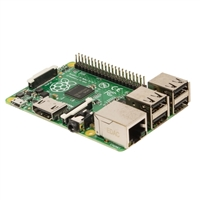
\includegraphics[width=300px,height=200px,keepaspectratio]{pi.jpg}
		\centering
	\end{center}

	\subsection{Advantages}

	The Raspberry Pi was a nicety in the following ways:

	\begin{itemize}
		\item Because the EE section has so many Raspberry Pi's, it was easy to get everyone up and running with a Linux distro very quickly.
		
		\item It created some more hands-on activity each day, letting the student put together their computer whenever they wanted to work (this doubles as negative)
	\end{itemize}

	\subsection{Disadvantages}

	Despite the benefits of using the small device, it was very easy to run into a few hiccups.

	\begin{itemize}
		\item Many students had trouble getting their VGA monitor to actually \textit{display}. This was a weekly occurrence. It typically took an instructor to intervene and try and remedy the problem themselves. 

		\item One student had struggled with the set up of the Raspberry Pi's so frequently that he went through four different devices in a day; myself and LCDR Wyman couldn't troubleshoot the first couple enough to get a display.
		
		\item Some operations on the Raspberry Pi are much slower considering its CPU power. Things like compiling software packages or installing software typically take a few minutes on the small chip, when on a typical Linux box they take only seconds.
		
		\item The Raspberry Pi initially has a different keyboard layout than what is used in the United States. Sure, we could cook solutions to this, but honestly you would be trying to solve a problem that doesn't have to be there in the first place.
	\end{itemize}

	\subsection{Future Recommendations}

	\paragraph{} I will take some author liberties here and actually recommend that for a future class that teaches Linux, make use of the Raspberry Pi only a temporary thing. In my opinion, for actual \textit{use} of the Linux operating system, it is more important to have a stable machine that they can quickly boot up and is much faster and has more modern repository packages. 

	\paragraph{} From a content-creator's perspective, the Raspberry Pi was a bit of a stumbling block. Myself being a Linux user, I run an Ubuntu Desktop on a typical Intel processor. Needless to say, this is the typical ``modern'' and ``mainstream'' Linux distribution that most old-Windows users convert to when they start to use Linux. Regardless, since I develop content in that environment, I would have to ``cross-check'' or verify success on the Raspbery Pi.  


	\begin{center}

		\graphicspath{ {.} }
		
\includegraphics[width=200px,height=200px,keepaspectratio]{ubuntu_logo.png}
		\centering

	\end{center}

	\paragraph{} There were a few occasions where I had compiled some binaries and forgot that the architecture was different on the Raspberry Pi, or didn't realize that some software package repositories weren't available on the Pi.

	\paragraph{} I cannot deny that the novelty of the Raspberry Pi is an attractive thing. In that regard I would recommend using it for maybe the first week of a future Linux class, but perhaps moving on to a more realistic environment for the users to learn on. 

	\subsection{Hardware \& Equipment}

	\paragraph{} So for the actual use of the Raspberry Pi, we needed a...

	\begin{itemize}
		\item 120-watt AC adapter
		\item Ethernet Cable
		\item HDMI-to-VGA adapter
		\item SD Card
		\item USB Mouse \& Keyboard
	\end{itemize}

	\subsection{Wireless Optional}

	\paragraph{} For the Raspberry Pi's, we used an Ethernet cable for wired Internet connection. You \textit{could} setup a wireless connection if you wanted to. I believe some of the newer models of the Raspberry Pi support wireless by default, but the models that we used for class we need a USB adapter, which would also have to be configured.

	\paragraph{} For scalability, I am unaware if it is feasible to automate the setup and configuration of the wireless USB adapter before installing the Raspbian image on the SD card... but afterwards, you could create a script to do what you need and push it out to the class by the github repo or any other means. You would have to trust the user-interaction and ask them to run the script, but you as the instructor can do obviously whatever you want. 

	\subsection{HDMI Output}

	\paragraph{} The monitors in the McAllister Hall Room 208 space that we used for this past semester only have DVI and VGA inputs. The Raspberry Pi models we were using only have an HDMI output. Because of this, we used an HDMI-to-VGA converter for every single device. This wasn't \textit{too much} of an issue; but it did add another step of troubleshooting when we couldn't get a display up on some students' device (which \textit{was} an issue).

	\paragraph{} If you care to remedy this you obviously have some options,  whether it be using a different room or different monitors or different devices entirely.

	\section{The Github Repository}

	\paragraph{} The Electrical Engineering department within the US Coast Guard Academy owns an academic license for \href{http://github.com}{http://github.com}, which allows the organization to create however many private and public repositories they would like.

	\paragraph{} This is taken advantage of in many other classes, but most others tend to really stumble when trying to push or pull content to and from github. The best way to manage digital content with github is through the command-line interface where command-line use was already an integral part of the Intro to Linux course. 

	\subsection{Students' Private Repositories}

	\paragraph{} Under the "MacEE" Github license, each student was able to their own private repository, typically titled with their last name (as an example, mine is \href{https://github.com/macee/Hammond}{https://github.com/macee/Hammond}). It was expected that students would have their own personal repository cloned and accessible in their Linux home directory. This was used to write reflections or post any code or files that was asked of the students during class. 

	\subsection{Class Public Repository}

	\paragraph{} For the 2016 Intro to Linux course, we created a specific \texttt{linux\_16} Github repository. This was made public and it housed all the code, content, and material for the course. As the content creator, this was what allowed me to easily push things to students computers. 

	\paragraph{} To adopt the Linux open-source mindset, it was my goal to ensure that repository was left public and included all of the source code and ``setup'' or ``build'' material, for everything we had done in class. I occasionally would remind students that all that content is there for their viewing pleasure, in case they were more curious how some of the training tools or the exercises worked --- but I am doubtful any students really dove deeper into it. On principle, anyway, I wanted it all to be available.


	


	%Throughout lab the last few weeks we have been building and analyzing a simple RC circuit, a low-pass filter with a $1500$ ohm ($\Omega$) resistor and a given capacitor. When we evaluated the theoretical math, we used a given value of a $0.1$ microfarad ($mF$) capacitor; however in within our experiment we unintentionally used a .$01 mF$ capacitor.


	\subsection{Create a Sandbox Environment}
	\label{Sandbox_Environment}

	Use a virtual machine
	take a snapshot before opening the e-mail and clicking the link/downloading the application
	take a snapshot after
	Look at the differences. RegShot, 

	\subsection{Save a copy of the phishing e-mail}
	\label{Save_a_copy}
	Get these things duplicaed, even on external harddrive


	\subsection{Replicate all external sources referred to}
	\label{Replicate all external sources}


	\section{Identify}
	\subsection{This is an All-Hands Evolution}
	We do not have any security professionals on site. Because of that, we rely on the entire Academy community to see and point out the malicious e-mails.

	\subsection{Determine who clicked the link}
	\subsection{Determine when the link was clicked}
	Establish a time frame and use that as the initial point for investigation.

	\subsection{Determine any other attack vectors}
	Who clicked on the link, when did they, what link/attachment, where were they in the network architecture, when did communication with the malicious server occer (is it beaconing back out?), where did the link direct the user (what website or server)

	what what when where etc.

	Try and determine the extent of the attack -- what is the skillset of the attacker --
	watch them for a little bit.

	\section{Containment}
	\subsection{Set up an Internet Filter}
	Block the link on the email using the web filter (Barracuda)

	Isolate them from the network if need be

	\subsection{Erase the E-mail}
	Remove these from the inboxes (only do this if all the steps previously have been taken care of)

	\subsection{Notify and Warn those affected}
	Tell the Academy what you have done.
	DO NOT SEND THIS MESSAGE OUT AS A CIO BULLETIN. Realistically, no one reads these.


	\section{Eradication \& Recovery}
	\subsection{Re-image affected user machines}
	\subsection{Blacklist malicious IP addresses}
	\subsection{Remind users they must handle their own data}


	\section{Develop an After-Action Report}
	\subsection{Document everything}

	\subsection{Formalize a Report}


	\section{Reflect on the Incident}
	\subsection{Assess your Team}

	Lessons Learned.
	Debrief. What was time consuming, how do you streamline the process.
	What went well?

	What tools do we lack (do we need any new kinds of scripts that we can develop in-house?)
	What went well, what should be continued

	Everyone should know their roles
		Who dumps pcaps from Security Onion?
		Who saves Snort logs?
		Who saves the e-mail?
		Who gathers event logs?
		Who oversees the operation?

	All in all, \textit{does each person have an individual job and are they following through?}

	\subsection{Review Network Architecture}
	\subsection{Future Mitigations}



	\section{What now?}

	\subsection{Get Involved}
	\subsection{Take off the Blindfolds}
	\subsection{Start the process all over again}

\end{document}